%!mode::"Tex:UTF-8"
\PassOptionsToPackage{unicode}{hyperref}
\PassOptionsToPackage{naturalnames}{hyperref}
\documentclass{article}
\usepackage{geometry}
%\usepackage{fullpage}
\usepackage{parskip}
\usepackage{physics}
\usepackage{amsmath}
\usepackage{amssymb}
\usepackage{xcolor}
\usepackage[colorlinks,linkcolor=blue,citecolor=green]{hyperref}
\usepackage{array}
\usepackage{longtable}
\usepackage{multirow}
\usepackage{comment}
\usepackage{graphicx}
\usepackage{cite}
\usepackage{amsfonts}
\usepackage{bm}
\usepackage{slashed}
\usepackage{dsfont}
\usepackage{mathtools}
\usepackage[compat=1.1.0]{tikz-feynman}
\usepackage{simplewick}
%\usepackage{fourier}
%\usepackage{slashbox}
%\usepackage{intent}
\usepackage{mathrsfs}
\usepackage{xparse}
\usepackage{enumerate}

\geometry{left=0.9cm,right=0.9cm,top=1.5cm,bottom=2cm}

\newcommand{\gm}{\gamma^{\mu}}
\newcommand{\gn}{\gamma^{\nu}}
\newcommand{\gs}{\gamma^{\sigma}}
\newcommand{\gr}{\gamma^{\rho}}
\newcommand{\gnr}{g^{\nu\rho}}
\newcommand{\gmr}{g^{\mu\rho}}
\newcommand{\gms}{g^{\mu\sigma}}
\newcommand{\gns}{g^{\nu\sigma}}
\newcommand{\vbp}{\vb{p}}
\newcommand{\vbk}{\vb{k}}
\newcommand{\g}{\gamma}
\renewcommand{\a}{\alpha}
\renewcommand{\b}{\beta}
\renewcommand{\t}{\theta}
\newcommand{\la}{\lambda}
\newcommand{\p}{\phi}
\newcommand{\vp}{\varphi}
\newcommand{\s}{\sigma}
\renewcommand{\G}{\Gamma}
\newcommand{\pars}{\slashed\partial}
\newcommand{\ps}{\slashed p}
\newcommand{\ks}{\slashed k}

\title{Homework: Quantum Field Theory \#8}
\author{Yingsheng Huang}
\begin{document}
\maketitle
{\bf1.}\quad
Yukawa theory.

\begin{enumerate}[(i)]
  \item $e^+e^-\rightarrow\mu^+\mu^-$. $H_I=\int\dd^3x[g_1\bar\psi_e\psi_e\phi+g_2\bar\psi_{\mu}\psi_{\mu}\phi]$, derive the $\mathcal{M}$ of the lowest order, calculate $\sum_{spins}\abs{\mathcal{M}}^2$ ,$\dv{\s}{\Omega}$ and $\s$.
  \begin{align*}
    iT&=\mel{kk'}{Te^{-i\Bqty{g_1\int\dd^4x\bar\psi_e\psi_e\phi+g_2\int\dd^4x\bar\psi_{\mu}\psi_{\mu}\phi}}}{pp'}\\
    &=\contraction[2.5ex]{}{\bra{k}}{k' g_2\int\dd^4x\bar\psi_{\mu}}{\psi_{\mu}}\contraction[1.5ex]{k}{\bra{k'}}{g_1\int\dd^4x}{\psi_{\mu}}\contraction[1.5ex]{\bra{kk'} g_2\int\dd^4x\bar\psi_{\mu}\psi_{\mu}}{\phi}{g_2\int\dd^4y\bar\psi_{e}\psi_{e}}{\phi}\contraction[2.5ex]{\bra{kk'} g_1\int\dd^4x\bar\psi_{\mu}\psi_{\mu}\phi  g_2\int\dd^4y}{\bar\psi}{_{e}\psi_{e}\phi p}{\ket{p'}}\contraction[3.5ex]{\bra{kk'} g_1\int\dd^4x\bar\psi_{\mu}\psi_{\mu}\phi  g_2\int\dd^4y\bar\psi_{e}}{\psi}{_{e}\phi}{\ket{p}}\bra{kk'} g_2\int\dd^4x\bar\psi_{\mu}\psi_{\mu}\phi  g_1\int\dd^4y\bar\psi_{e}\psi_{e}\phi \ket{pp'}\\
    &=g_1g_2\int\dd^4x\dd^4y\bar u_{\mu}^se^{ik\cdot x}v^{s'}_{\mu}e^{ik'\cdot x}\int\frac{\dd^4q}{(2\pi)^4}\frac{i}{q^2-m^2}e^{-iq\cdot(x-y)}\bar v^re^{-ip'\cdot y}u^{r'}e^{-ip\cdot y}\\
    &=g_1g_2\bar u_{\mu}^sv^{s'}_{\mu}\int\frac{\dd^4q}{(2\pi)^4}\frac{i}{q^2-m^2}\bar v^ru^{r'}(2\pi)^4\delta^4(k+k'-q)(2\pi)^4\delta^4(q-p-p')\\
    &=\bar u^s(k)g_2v^{s'}(k')\frac{i}{(p+p')^2-m^2}\bar v^r(p')g_1u^{r'}(p)(2\pi)^4\delta^4(p+p'-k-k')
  \end{align*}
  And the feynman diagram
  \begin{center}
    \feynmandiagram[large, horizontal=x to y]{
    i1[particle=$e^-$] -- [fermion,momentum={\(p\)}] x-- [fermion,rmomentum={\(p'\)}] i2[particle=$e^+$],
    x -- [scalar,momentum={\(q\)}] y,
    f1[particle=$\mu^-$] -- [fermion,rmomentum={\(k\)}] y -- [fermion,momentum={\(k'\)}] f2[particle=$\mu^+$],
    };
  \end{center}
  The scattering amplitude
  $$i\mathcal{M}=\bar u^s(k)g_2v^{s'}(k')\frac{i}{q^2-m^2}\bar v^r(p')g_1u^{r'}(p)$$
  where $q=p+p'$.
  And
  $$\dv{\s}{\Omega}|_{CM}=\frac{1}{2E_p2E_{p'}\abs{v_p-v_{p'}}}\frac{\abs{\vb{k}}}{(2\pi)^24E_{CM}}\abs{\mathcal{M}}^2$$
  The spin sum amplitude
  \begin{align*}
    \sum_{spins}\abs{\mathcal{M}}^2&=\sum_{spins}g_1^2g_2^2[\bar u^s(k)v^{s'}(k')\frac{1}{q^2-m^2}\bar v^r(p')u^{r'}(p)][\bar u^s(k)v^{s'}(k')\frac{1}{q^2-m^2}\bar v^r(p')u^{r'}(p)]^*\\
    &=\sum_{spins}g_1^2g_2^2[\bar u^s(k)v^{s'}(k')\frac{1}{q^2-m^2}\bar v^r(p')u^{r'}(p)][\bar v^{s'}(k')u^s(k)\frac{1}{q^2-m^2}\bar u^{r'}(p)v^r(p')]\\
    &=\sum_{spins}\frac{g_1^2g_2^2}{(q^2-m^2)^2}\tr{u^s(k)\bar u^s(k)v^{s'}(k')\bar v^{s'}(k')}\tr{v^r(p')\bar v^r(p')u^{r'}(p)\bar u^{r'}(p)}\\
    &=\frac{g_1^2g_2^2}{(q^2-m^2)^2}\tr{(\ks+m_{\mu})(\ks'-m_{\mu})}\tr{(\ps'-m_e)(\ps+m_e)}\\
    &=\frac{g_1^2g_2^2}{(q^2-m^2)^2}(4k\cdot k'-m_{\mu}^2)(4p\cdot p'-m_e^2)
  \end{align*}
  Now we know that in centre-of-mass frame
  $$p^{\mu}=(E,0,0,p),{p'}^{\mu}=(E,0,0,-p),k^{\mu}=(E,k\sin\theta,0,k\cos\theta),{k'}^{\mu}=(E,-k\sin\theta,0,-k\cos\theta)$$
  so
  $$p\cdot p'=E^2+p^2,k\cdot k'=E^2+k^2,p^2=E^2-m_e^2,k^2=E^2-m_{\mu}^2,E_{CM}=2E,q^2=4E^2=s$$
  Thus
  \begin{align*}
    \frac{1}{4}\sum_{spins}\abs{\mathcal{M}}^2&=\frac{g_1^2g_2^2}{4(q^2-m^2)^2}(8E^2-5m^2_e)(8E^2-5m_{\mu}^2)
  \end{align*}
  The differential cross section is (the mass of electron is neglected)
  \begin{align*}
    \dv{\s}{\Omega}|_{CM}&=\frac{1}{2E_p2E_{p'}\abs{v_p-v_{p'}}}\frac{\abs{\vb{k}}}{(2\pi)^24E_{CM}}\frac{1}{4}\sum_{spins}\abs{\mathcal{M}}^2\\
    &=\frac{1}{2E^2_{CM}}\frac{k}{16\pi^2E_{CM}}\frac{g_1^2g_2^2}{4(q^2-m^2)^2}8E^2(8E^2-5m_{\mu}^2)\\
    &=\frac{\sqrt{E^2-m_{\mu}^2}}{16\pi^2s}\frac{g_1^2g_2^2}{4(s-m^2)^2}(8E^2-5m_{\mu}^2)\\
    &=\frac{\sqrt{s-4m_{\mu}^2}}{128\pi^2s}\frac{g_1^2g_2^2}{(s-m^2)^2}(2s-5m_{\mu}^2)
  \end{align*}
  and total cross section
  $$\s=\frac{\sqrt{s-4m_{\mu}^2}}{32\pi s}\frac{g_1^2g_2^2}{(s-m^2)^2}(2s-5m_{\mu}^2)$$
  \item NR scattering.
  \begin{enumerate}[(a)]
    \item $ff\rightarrow ff$.
    \begin{equation*}
      \feynmandiagram[baseline={(y.base)},vertical=x to y]{
      i1[particle=f \(\bar u\)]--[anti fermion]x--[scalar]y--[anti fermion]i2[particle=f \(u\)],
      f1[particle=f \(u\)]--[fermion]x--[scalar]y--[fermion]f2[particle=f \(\bar u\)],
      };
      =(-g^2)[\bar u(k) u(p)\frac{i}{q^2-M^2}\bar u(k')u(p')-\bar u(k') u(p)\frac{i}{q^2-M^2}\bar u(k)u(p')]
    \end{equation*}
    %\begin{align*}
    %  \frac{1}{4}\sum_{spins}\abs{\mathcal{M}}^2&=\frac{1}{4}\tr{(\ks+m)(\ps+m)}\frac{1}{(q^2-M^2)^2}\tr{(\ks'+m)(\ps'+m)}\\
    %  &=\frac{1}{4(q^2-M^2)^2}(4k\cdot p+m^2)(4k'\cdot p'+m^2)\\
    %  \intertext{In centre-of-mass frame}
    %  &=\frac{(4E^2-4\abs{\vb{p}}\abs{\vb{k}}\cos\theta+m^2)^2}{4(q^2-M^2)^2}\\
    %  &=\frac{[4\abs{\vb{p}}^2(1-\cos\theta)+4m^2]^2}{4(q^2-M^2)^2}\\
    %  &=\frac{4[\abs{\vb{p}}^2(1-\cos\theta)+m^2]^2}{(s-M^2)^2}
    %\end{align*}
    %\begin{align*}
    %  \dv{\s}{\cos\theta}&=\frac{\frac{1}{4}\sum_{spins}\abs{\mathcal{M}}^2}{32\pi s}=\frac{[\abs{\vb{p}}^2(1-\cos\theta)+m^2]^2}{8\pi s(s-M^2)^2}
    %\end{align*}
    %\begin{align*}
    %  \s=\frac{2 m^4+4 m^2 p^2+\frac{8 p^4}{3}}{8\pi s(s-M^2)^2}=\frac{4 m^4-2 m^2 s+s^2}{48\pi s(s-M^2)^2}
    %\end{align*}
    Use Yukawa potential
    $$i\mathcal{M}=(-g^2)[\bar u(k) u(p)\frac{i}{q^2-M^2}\bar u(k')u(p')-\bar u(k') u(p)\frac{i}{q^2-M^2}\bar u(k)u(p')]$$
    For non-relativistic limit ($p=(m,\vb{p})$ and so on)
    $$\bar u^s(k)u^r(p)=2m\delta^{sr}$$
    and so on. So
    $$i\mathcal{M}=(-g^2)[\frac{i}{\vb{(k-p)}^2-M^2}2m\delta^{rs}2m\delta^{r's'}-\frac{i}{\vb{(k'-p)}^2-M^2}2m\delta^{r's}2m\delta^{rs'}]$$
    And in Born approximation
    $$\mel{p'}{iT}{p}=-i\tilde V(\vb{q})(2\pi)\delta^4(E_{\vb{p'}}-E_{\vb{p}})$$
    Comparing with the former one we have for each $\vb{q}$
    $$\tilde V(\vb{q})=(-g^2)[\frac{i}{\vb{q}^2-M^2}$$
    \item $f\bar f\rightarrow f\bar f$.
    \begin{align*}
      \feynmandiagram[horizontal=x to y, baseline=(x.base)]{
      i1[particle=f]--[fermion]x--[fermion] i2[particle={\(\bar f\)}],
      x--[scalar]y,
      f1[particle={\(\bar f\)}]--[fermion]y--[fermion]f2[particle=f],
      };=(-g^2)\bar u(k) v(k') \frac{i}{q^2-M^2}\bar v(p') u(p)
    \end{align*}
    %$$\frac{1}{4}\sum_{spins}\abs{\mathcal{M}}^2=\frac{1}{4}\tr{(\ks+m)(\ks'-m)}\frac{1}{(q^2-M^2)^2}\tr{(\ps+m)(\ps'-m)}=\frac{1}{4(q^2-M^2)^2}(4k\cdot k'-m^2)(4p\cdot p'-m^2)$$
    %$$\dv{\s}{\cos\theta}=\frac{\frac{1}{4}\sum_{spins}\abs{\mathcal{M}}^2}{32\pi s}=\frac{(2s-5m^2)^2}{128\pi s}$$
    %$$\s=\frac{(2s-5m^2)^2}{64\pi s}$$
    Similarly to the discussion we made before, the sign of the potential in Born approximation is entirely dependent on the vertex. So it's again attractive.
  \end{enumerate}
\end{enumerate}

{\bf2.}\quad
Trace technology.
\begin{enumerate}[(i)]
  \item $\tr{\g^5}$
  \begin{align*}
    \tr{\g^5}&=i\tr{\g^0\g^1\g^2\g^3}\\
    &=4i(g^{01}g^{23}-g^{02}g^{13}+g^{03}g^{12})\\
    &=0
  \end{align*}
  \item $\tr{\g^5\gm\gn}$
  \begin{align*}
    \tr{\g^5\gm\gn}&=\tr{\g^0\g^0\g^5\gm\gn}\\
    &=\tr{\g^0\g^5\gm\gn\g^0}\\
    \intertext{note that $\tr{\g^5\gn\g^0}=\tr{\g^1\g^2\g^3\gn}=0$}
    &=(-1)^3\tr{\g^5\gm\gn\g^0\g^0}\\
    &=-\tr{\g^5\gm\gn}\\
    &=0
  \end{align*}
  \item $\tr{\g^5\gm\gn\gr\gs}$

  For a proof of identity 6, the same trick still works unless $ {\displaystyle (\mu \nu \rho \sigma )\,}$ is some permutation of (0123), so that all 4 gammas appear. The anticommutation rules imply that interchanging two of the indices changes the sign of the trace, so $ {\displaystyle \operatorname {tr} (\gamma ^{\mu }\gamma ^{\nu }\gamma ^{\rho }\gamma ^{\sigma }\gamma ^{5})\,}$ must be proportional to ${\displaystyle \epsilon ^{\mu \nu \rho \sigma }\,}$$ {\displaystyle (\epsilon ^{0123}=\eta ^{0\mu }\eta ^{1\nu }\eta ^{2\rho }\eta ^{3\sigma }\epsilon _{\mu \nu \rho \sigma }=\eta ^{00}\eta ^{11}\eta ^{22}\eta ^{33}\epsilon _{0123}=-1)\,}$. The proportionality constant is ${\displaystyle 4i\,}$, as can be checked by plugging in $ {\displaystyle (\mu \nu \rho \sigma )=(0123)\,} $, writing out $ {\displaystyle \gamma ^{5}\,}$, and remembering that the trace of the identity is 4.
  %\begin{align*}
  %  \tr{\g^5\gm\gn\gr\gs}&=2g^{\rho\s}\tr{\g^5\gm\gn}-\tr{\g^5\gm\gn\gs\gr}\\
  %  &=2g^{\rho\s}\tr{\g^5\gm\gn}-2g^{\s\nu}\tr{\g^5\gm\gr}+\tr{\g^5\gm\gs\gn\gr}\\
  %  &=2g^{\rho\s}\tr{\g^5\gm\gn}-2g^{\s\nu}\tr{\g^5\gm\gr}+2g^{\s\mu}\tr{\g^5\gn\gr}-\tr{\g^5\gs\gm\gn\gr}\\
  %  &=2g^{\rho\s}\tr{\g^5\gm\gn}-2g^{\s\nu}\tr{\g^5\gm\gr}+2g^{\s\mu}\tr{\g^5\gn\gr}+\tr{\gs\g^5\gm\gn\gr}
  %\end{align*}
  \begin{align*}
    \tr{\g^5\gm\gn\gr\gs}&=\tr{\g^0\g^0\g^5\gm\gn\gr\gs}\\
    &=-\tr{\g^0\g^5\g^0\gm\gn\gr\gs}\\
    &=-2g^{0\mu}\tr{\g^0\g^5\gn\gr\gs}+\tr{\g^0\g^5\gm\g^0\gn\gr\gs}\\
    &=-2g^{0\mu}\tr{\g^0\g^5\gn\gr\gs}+2g^{0\nu}\tr{\g^0\g^5\gm\gr\gs}-\tr{\g^0\g^5\gm\gn\g^0\gr\gs}\\
    &=-2g^{0\mu}\tr{\g^0\g^5\gn\gr\gs}+2g^{0\nu}\tr{\g^0\g^5\gm\gr\gs}-2g^{0\rho}\tr{\g^0\g^5\gm\gn\gs}+\tr{\g^0\g^5\gm\gn\gr\g^0\gs}\\
    &=-2g^{0\mu}\tr{\g^0\g^5\gn\gr\gs}+2g^{0\nu}\tr{\g^0\g^5\gm\gr\gs}-2g^{0\rho}\tr{\g^0\g^5\gm\gn\gs}+2g^{0\s}\tr{\g^0\g^5\gm\gn\gr}\\&-\tr{\g^0\g^5\gm\gn\gr\gs\g^0}\\
    &=-2g^{0\mu}\tr{\g^0\g^5\gn\gr\gs}+2g^{0\nu}\tr{\g^0\g^5\gm\gr\gs}-2g^{0\rho}\tr{\g^0\g^5\gm\gn\gs}+2g^{0\s}\tr{\g^0\g^5\gm\gn\gr}\\&-\tr{\g^5\gm\gn\gr\gs}\\
    &=-g^{0\mu}\tr{\g^0\g^5\gn\gr\gs}+g^{0\nu}\tr{\g^0\g^5\gm\gr\gs}-g^{0\rho}\tr{\g^0\g^5\gm\gn\gs}+g^{0\s}\tr{\g^0\g^5\gm\gn\gr}
  \end{align*}
  For $\tr{\g^0\g^5\gn\gr\gs}$
  \begin{align*}
    \tr{\g^0\g^5\gn\gr\gs}&=-\tr{g^1\g^1\g^0\g^5\gn\gr\gs}\\
    &=-2g^{1\nu}\tr{\g^1\g^0\g^5\gr\gs}+2g^{1\rho}\tr{\g^1\g^0\g^5\gn\gs}-2g^{1\s}\tr{\g^1\g^0\g^5\gn\gr}+\tr{\g^1\g^1\g^5\gn\gr\gs}\\
    &=-g^{1\nu}\tr{\g^1\g^0\g^5\gr\gs}+g^{1\rho}\tr{\g^1\g^0\g^5\gn\gs}-g^{1\s}\tr{\g^1\g^0\g^5\gn\gr}
  \end{align*}
  For $\tr{\g^1\g^0\g^5\gr\gs}$
  \begin{align*}
    \tr{\g^1\g^0\g^5\gr\gs}&=-\tr{\g^2\g^2\g^1\g^0\g^5\gr\gs}\\
    &=\tr{\g^2\g^1\g^0\g^5\g^2\gr\gs}\\
    &=2g^{2\rho}\tr{\g^2\g^1\g^0\g^5\gs}-2g^{2\s}\tr{\g^2\g^1\g^0\g^5\gr}+\tr{\g^2\g^2\g^1\g^0\g^5\gr\gs}\\
    &=g^{2\rho}\tr{\g^2\g^1\g^0\g^5\gs}-g^{2\s}\tr{\g^2\g^1\g^0\g^5\gr}
  \end{align*}
  For $\tr{\g^2\g^1\g^0\g^5\gs}$
  \begin{align*}
    \tr{\g^2\g^1\g^0\g^5\gs}&=-\tr{\g^3\g^3\g^2\g^1\g^0\g^5\gs}\\
    &=-\tr{\g^3\g^2\g^1\g^0\g^5\g^3\gs}\\
    &=-g^{3\s}\tr{\g^3\g^2\g^1\g^0\g^5}\\
    &=-ig^{3\s}
  \end{align*}
  Put these back and
  \begin{align*}
    \tr{\g^1\g^0\g^5\gr\gs}&=g^{2\rho}\tr{\g^2\g^1\g^0\g^5\gs}-g^{2\s}\tr{\g^2\g^1\g^0\g^5\gr}\\
    &=-ig^{2\rho}g^{3\s}+ig^{2\s}g^{3\rho}
  \end{align*}
  \begin{align*}
    \tr{\g^0\g^5\gn\gr\gs}&=-g^{1\nu}\tr{\g^1\g^0\g^5\gr\gs}+g^{1\rho}\tr{\g^1\g^0\g^5\gn\gs}-g^{1\s}\tr{\g^1\g^0\g^5\gn\gr}\\
    &=-g^{1\nu}(-g^{2\rho}g^{3\s}+g^{2\s}g^{3\rho})+g^{1\rho}(-g^{2\nu}g^{3\s}+g^{2\s}g^{3\nu})-g^{1\s}(-g^{2\nu}g^{3\rho}+g^{2\rho}g^{3\nu})\\
    &=ig^{1\nu}g^{2\rho}g^{3\s}-ig^{1\nu}g^{2\s}g^{3\rho}-ig^{1\rho}g^{2\nu}g^{3\s}+ig^{1\rho}g^{2\s}g^{3\nu}+ig^{1\s}g^{2\nu}g^{3\rho}-ig^{1\s}g^{2\rho}g^{3\nu}
  \end{align*}
  \begin{align*}
    \tr{\g^5\gm\gn\gr\gs}&=-g^{0\mu}\tr{\g^0\g^5\gn\gr\gs}+g^{0\nu}\tr{\g^0\g^5\gm\gr\gs}-g^{0\rho}\tr{\g^0\g^5\gm\gn\gs}+g^{0\s}\tr{\g^0\g^5\gm\gn\gr}\\
    &=-ig^{0\mu}(g^{1\nu}g^{2\rho}g^{3\s}-g^{1\nu}g^{2\s}g^{3\rho}-g^{1\rho}g^{2\nu}g^{3\s}+g^{1\rho}g^{2\s}g^{3\nu}+g^{1\s}g^{2\nu}g^{3\rho}-g^{1\s}g^{2\rho}g^{3\nu})\\
    &\phantom{=}+ig^{0\nu}(g^{1\mu}g^{2\rho}g^{3\s}-g^{1\mu}g^{2\s}g^{3\rho}-g^{1\rho}g^{2\mu}g^{3\s}+g^{1\rho}g^{2\s}g^{3\mu}+g^{1\s}g^{2\mu}g^{3\rho}-g^{1\s}g^{2\rho}g^{3\mu})\\
    &\phantom{=}-ig^{0\rho}(g^{1\mu}g^{2\nu}g^{3\s}-g^{1\mu}g^{2\s}g^{3\nu}-g^{1\nu}g^{2\mu}g^{3\s}+g^{1\nu}g^{2\s}g^{3\mu}+g^{1\s}g^{2\mu}g^{3\nu}-g^{1\s}g^{2\nu}g^{3\mu})\\
    &\phantom{=}+ig^{0\s}(g^{1\mu}g^{2\nu}g^{3\rho}-g^{1\mu}g^{2\rho}g^{3\nu}-g^{1\nu}g^{2\mu}g^{3\rho}+g^{1\nu}g^{2\rho}g^{3\mu}+g^{1\rho}g^{2\mu}g^{3\nu}-g^{1\rho}g^{2\nu}g^{3\mu})\\
    &=-4i\epsilon^{\mu\nu\rho\s}
  \end{align*}
  (Use the identity mentioned before.)
  %Similarly, plug in a pair of $\g^0$ and it should give 5 minus signs. So it's zero again.
\end{enumerate}

{\bf3.}\quad
The electron muon scattering process $e^-\mu^-\rightarrow e^-\mu^-$.

We can plot the feynman diagram and give the invariant amplitude
$$\feynmandiagram[vertical=x to y]{
i1[particle=\(e^-\)]--[anti fermion, rmomentum=\(p'\)]x--[photon]y--[anti fermion,rmomentum=\(k\)]f2[particle=\(\mu^-\)],
i2[particle=\(e^-\)]--[fermion,momentum=\(p\)]x--[photon]y--[fermion, momentum=\(k'\)]f1[particle=\(\mu^-\)],
};$$
$$i\mathcal{M}=(ie^2)\bar u^s(p)\gm u^{s'}(p')\frac{g_{\mu\nu}}{q^2}\bar u^{r}(k)\gn u^{r}(k')$$
The spin sum amplitude
\begin{align*}
  \frac{1}{4}\sum_{spins}\abs{\mathcal{M}}^2&=\frac{e^4}{4q^4}\tr{(\ps+m_e)\gm(\ps'+m_e)\gn}\tr{(\ks+m_{\mu})\g_{\mu}(\ks'+m_{\mu})\g_{\nu}}\\
  &=\frac{e^4}{4q^4}[4(p^{\mu} p'^{\nu}+p'^{\mu}p^{\nu}-p\cdot p'g^{\mu\nu})+4m_e^2g^{\mu\nu}][4(k^{\mu}k'^{\nu}+k'^{\mu}k^{\nu}-k\cdot k'g_{\mu\nu})+4m_{\mu}^2g_{\mu\nu}]\\
  &=\frac{4e^4}{q^4}[p^{\mu} p'^{\nu}+p'^{\mu}p^{\nu}-p\cdot p'g^{\mu\nu}+m_e^2g^{\mu\nu}][k^{\mu}k'^{\nu}+k'^{\mu}k^{\nu}-k\cdot k'g_{\mu\nu}+m_{\mu}^2g_{\mu\nu}]\\
  \intertext{ignore the electron mass $m_e$}
  &=\frac{4e^4}{q^4}[p^{\mu} p'^{\nu}+p'^{\mu}p^{\nu}-p\cdot p'g^{\mu\nu}][k^{\mu}k'^{\nu}+k'^{\mu}k^{\nu}-k\cdot k'g_{\mu\nu}+m_{\mu}^2g_{\mu\nu}]\\
  &=\frac{4e^4}{q^4}[(p\cdot k)(p'\cdot k')+(p\cdot k')(p'\cdot k)-(p\cdot p')(k\cdot k')+m_{\mu}^2(p\cdot p')+(p'\cdot k)(p\cdot k')+(p'\cdot k')(p\cdot k)-(p'\cdot p)(k\cdot k')\\
  &+m_{\mu}^2(p'\cdot p)-(p\cdot p')(k\cdot k')-(p\cdot p')(k\cdot k')+4(p\cdot p')(k\cdot k')-4m^2_{\mu}(p\cdot p')]\\
  &=\frac{8e^4}{q^4}[(p\cdot k)(p'\cdot k')+(p\cdot k')(p'\cdot k)-m_{\mu}^2(p\cdot p')]
\end{align*}
where $q=p'-p$.

The differential cross section ($\theta$ is the angle between the initial muon and final muon, and in centre-of-mass frame)
\begin{align*}
  \dv{\s}{\Omega}|_{CM}&=\frac{1}{2E_p2E_{k}\abs{v_p-v_{k}}}\frac{\abs{\vb{p'}}}{(2\pi)^24E_{CM}}\frac{1}{4}\sum_{spins}\abs{\mathcal{M}}^2\\
  \intertext{for our problem we set $\abs{v_p-v_{k}}=1$ first and we'll plug it back later, $E_{p}=\omega$}
  &=\frac{1}{2\omega2E_{k}}\frac{\abs{\vb{p'}}}{(2\pi)^24E_{CM}}\frac{8e^4}{q^4}[(p\cdot k)(p'\cdot k')+(p\cdot k')(p'\cdot k)-m_{\mu}^2(p\cdot p')]\\
  \intertext{and $$p=(\omega,\omega\hat z), k=(E_k,-\omega\hat z), p'=(\omega_{p'},\vb{\omega_{p'}}), k'=(E_{k'},-\vb{\omega_{p'}}),\vb{\omega_{p'}}=(-\omega_{p'}\sin\theta,0,-\omega_{p'}\cos\theta)$$ which explicitly is $$p=(\omega,\omega\hat z), k=(E_k,-\omega\hat z), p'=(\omega_{p'},-\omega_{p'}\sin\theta,0,-\omega_{p'}\cos\theta), k'=(E_{k'},\omega_{p'}\sin\theta,0,\omega_{p'}\cos\theta)$$so $$p\cdot k=\omega E_k+\omega^2, p'\cdot k'=\omega_{p'}(\omega+E_k), E_k^2=\omega^2+m_{\mu}^2, p\cdot k'=\omega^2+\omega E_k-\omega\omega_{p'}-\omega\omega_{p'}\cos\theta, p'\cdot k=\omega_{p'}E_k-\omega\omega_{p'}\cos\theta$$$$p\cdot p'=\omega\omega_{p'}(1+\cos\theta), q^2=(p'-p)^2=2\omega_{p'}\omega(1-\cos\theta)$$and gives}
  &=\frac{1}{2\omega2E_{k}}\frac{\abs{\vb{p'}}}{(2\pi)^24E_{CM}}\frac{8e^4}{q^4}[(\omega E_k+\omega^2)(\omega_{p'}(\omega+E_k))+(\omega^2+\omega E_k-\omega\omega_{p'}-\omega\omega_{p'}\cos\theta)(\omega_{p'}E_k-\omega\omega_{p'}\cos\theta)\\&-m_{\mu}^2(\omega\omega_{p'}(1+\cos\theta))]\\
  &=\frac{1}{2\omega2E_{k}}\frac{\abs{\vb{p'}}}{(2\pi)^24E_{CM}}\frac{8e^4}{q^4}[\omega E_k\omega_{p'}\omega+\omega E_k\omega_{p'}E_k+\omega^2\omega_{p'}\omega+\omega^2\omega_{p'}E_k+\omega^2\omega_{p'}E_k-\omega^2\omega\omega_{p'}\cos\theta+\omega E_k\omega_{p'}E_k\\
  &-\omega E_k\omega\omega_{p'}\cos\theta-\omega\omega_{p'}\omega_{p'}E_k+\omega\omega_{p'}\omega\omega_{p'}\cos\theta-\omega\omega_{p'}\cos\theta\omega_{p'}E_k+\omega\omega_{p'}\cos\theta\omega\omega_{p'}\cos\theta-m_{\mu}^2\omega\omega_{p'}(1+\cos\theta)\\
  &=\frac{1}{2\omega2E_{k}}\frac{\omega_{p'}}{(2\pi)^24(\omega+E_k)}\frac{8e^4}{q^4}[3\omega^2 E_k\omega_{p'}+2\omega E_k^2\omega_{p'}+\omega^3\omega_{p'}-\omega^3\omega_{p'}\cos\theta-\omega^2 E_k\omega_{p'}\cos\theta-\omega\omega_{p'}^2E_k(1+\cos\theta)+\omega^2\omega_{p'}^2\cos\theta\\&+\omega^2\omega_{p'}^2\cos^2\theta-m_{\mu}^2\omega\omega_{p'}(1+\cos\theta)]\\
  \intertext{assuming no large change in energy and gives $\omega_{p'}=\omega$, so}
  &=\frac{1}{2\omega2E_{k}}\frac{\omega}{(2\pi)^24(\omega+E_k)}\frac{8e^4}{q^4}[2\omega^3 E_k+2\omega^2 E_k^2+\omega^4-2\omega^3 E_k\cos\theta+\omega^4\cos^2\theta-m_{\mu}^2\omega^2(1+\cos\theta)]\\
  &=\frac{1}{2\omega2E_{k}}\frac{\omega}{(2\pi)^24(\omega+E_k)}\frac{2e^4}{\omega^4(1-\cos\theta)^2}[2\omega^3 E_k+2\omega^2 E_k^2+\omega^4-2\omega^3 E_k\cos\theta+\omega^4\cos^2\theta-m_{\mu}^2\omega^2(1+\cos\theta)]\\
  &=\frac{1}{2\omega2E_{k}}\frac{\omega}{(2\pi)^24(\omega+E_k)}\frac{2e^4}{\omega^2(1-\cos\theta)^2}[2\omega E_k+2 E_k^2+\omega^2-2\omega E_k\cos\theta+\omega^2\cos^2\theta-m_{\mu}^2(1+\cos\theta)]\\
  &=\frac{1}{2\omega2E_{k}}\frac{\omega}{(2\pi)^24(\omega+E_k)}\frac{2e^4}{\omega^2(1-\cos\theta)^2}[(E_k+\omega)^2+(E_k-\omega\cos\theta)^2-m_{\mu}^2(1+\cos\theta)]\\
  \intertext{plug in $\abs{v_p-v_{k}}=\abs{1+\frac{\omega}{E_k}}$}
  &=\frac{1}{2\omega2E_{k}\abs{1+\frac{\omega}{E_k}}}\frac{\omega}{(2\pi)^24(\omega+E_k)}\frac{2e^4}{\omega^2(1-\cos\theta)^2}[(E_k+\omega)^2+(E_k-\omega\cos\theta)^2-m_{\mu}^2(1+\cos\theta)]\\
  &=\frac{1}{4\abs{E_k+\omega }}\frac{1}{(2\pi)^24(\omega+E_k)}\frac{2e^4}{\omega^2(1-\cos\theta)^2}[(E_k+\omega)^2+(E_k-\omega\cos\theta)^2-m_{\mu}^2(1+\cos\theta)]\\
  &=\frac{1}{64\pi^2(\omega+E_k)^2}\frac{2e^4}{\omega^2(1-\cos\theta)^2}[(E_k+\omega)^2+(E_k-\omega\cos\theta)^2-m_{\mu}^2(1+\cos\theta)]\\  &=\frac{1}{2(\omega+E_k)^2}\frac{\alpha^2}{\omega^2(1-\cos\theta)^2}[(E_k+\omega)^2+(E_k-\omega\cos\theta)^2-m_{\mu}^2(1+\cos\theta)]
\end{align*}
where $E_k=\sqrt{\omega^2+m_{\mu}^2}$.

In high energy limit $m_{\mu}\rightarrow 0$
\begin{align*}
  \dv{\s}{\Omega}|_{CM}&=\frac{1}{2E_{CM}^2}\frac{\alpha^2}{(1-\cos\theta)^2}[4+(1-\cos\theta)^2]
\end{align*}

%We find this way the cross section is very complicated. So we now invoke the crossing symmetry:
%$$p\rightarrow p,k\rightarrow -k,p'\rightarrow -p',k'\rightarrow k'$$
%and earlier we know that
%$$p^{\mu}=(E,0,0,p),{p'}^{\mu}=(E,0,0,-p),k^{\mu}=(E,k\sin\theta,0,k\cos\theta),{k'}^{\mu}=(E,-k\sin\theta,0,-k\cos\theta)$$
%so after applying crossing symmetry
%$$p^{\mu}=(E,0,0,p),{p'}^{\mu}=(E,0,0,p),k^{\mu}=(E,-k\sin\theta,0,-k\cos\theta),{k'}^{\mu}=(E,-k\sin\theta,0,-k\cos\theta)$$
%$$p\cdot p'=E^2-p^2,k\cdot k'=E^2+k^2,p^2=E^2-m_e^2,k^2=E^2-m_{\mu}^2,E_{CM}=2E,q^2=4E^2=s$$

{\bf4.}\quad
Feynman diagrams.
\begin{enumerate}[(i)]
  \item $e^-e^-\rightarrow e^-e^-$
  \begin{align*}
    \feynmandiagram[vertical=x to y]{
    i1[particle=$e^-$]--[anti fermion]x--[anti fermion]f1[particle=$e^-$],
    x--[photon]y,
    i2[particle=$e^-$]--[anti fermion]y--[anti fermion]f2[particle=$e^-$],
    };
    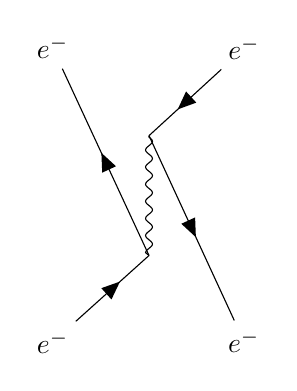
\begin{tikzpicture}
      \begin{feynman}
        \diagram [vertical'=a to b] {
        i1 [particle=\(e^{-}\)]
        -- [fermion] a
        -- [draw=none] f1 [particle=\(e^{-}\)],
        a -- [photon] b,
        i2 [particle=\(e^{-}\)]
        -- [fermion] b
        -- [draw=none] f2 [particle=\(e^{-}\)],
        };
        \diagram* {
        (a) -- [fermion] (f2),
        (b) -- [fermion] (f1),
        };
      \end{feynman}
    \end{tikzpicture}
  \end{align*}
  \item $e^-e^+\rightarrow e^-e^+$
  \begin{align*}
    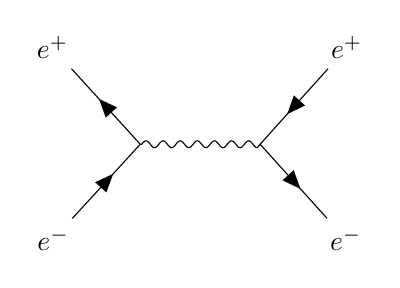
\begin{tikzpicture}
      \begin{feynman}
      \diagram[horizontal=x to y]{
      i1[particle=$e^-$]--[fermion]x--[fermion]i2[particle=$e^+$],
      x--[photon]y,
      f1[particle=$e^+$]--[fermion]y--[fermion]f2[particle=$e^-$],
      };
      \end{feynman}
    \end{tikzpicture}
    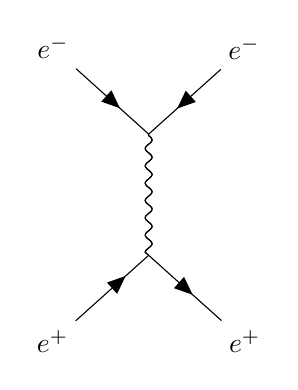
\begin{tikzpicture}
      \begin{feynman}
      \diagram[vertical=x to y]{
      i1[particle=$e^-$]--[fermion]x--[photon]y--[fermion]f2[particle=$e^+$],
      f1[particle=$e^-$]--[fermion]x--[photon]y--[anti fermion]i2[particle=$e^+$],
      };
      \end{feynman}
    \end{tikzpicture}
  \end{align*}
\end{enumerate}

{\bf5.}\quad
Verify Ward identity. (Use condition (i) and (ii) and abtain the result $\mathcal{M}=0$ which verified Ward identity.)

We already have the invariant amplitude as follows
$$i\mathcal{M}=-ie^2\epsilon^*_{\mu}(k')\epsilon_{\nu}(k)\bar u(p')[\frac{\gm\ks\gn+2\gm p^{\nu}}{2p\cdot k}+\frac{\gn\ks'\gm-2\gn p^{\mu}}{2p\cdot k'}]u(p)$$
and from the feynman diagram
\begin{align*}
  \feynmandiagram[horizontal=x to y,baseline=(x.base)]{
  i1--[fermion,momentum=p]x--[fermion]y--[fermion,momentum=p']f2,
  i2--[photon,momentum=k]x,
  y--[photon,momentum=k']f1,
  };+\feynmandiagram[horizontal=x to y,baseline=(x.base)]{
  i1--[fermion,momentum=p]x--[fermion]y--[fermion,momentum=p']f2,
  i2--[photon,rmomentum=k']x,
  y--[photon,rmomentum=k]f1,
  };
\end{align*}
we have
$$p+k=p'+k',k^2=k'^2=0$$
And note that from Dirac equation
$$\ps u(p)=mu(p)$$
$$\bar u(p)\ps=m\bar u(p)$$
\begin{enumerate}[(i)]
  \item $\epsilon^*_{\mu}(k')\rightarrow k'_{\mu}$
  \begin{align*}
    i\mathcal{M}&=-ie^2k'_{\mu}\epsilon_{\nu}(k)\bar u(p')[\frac{\gm\ks\gn+2\gm p^{\nu}}{2p\cdot k}+\frac{\gn\ks'\gm-2\gn p^{\mu}}{2p\cdot k'}]u(p)\\
    &=-ie^2\epsilon_{\nu}(k)\bar u(p')[\frac{\ks'\ks\gn+2\ks' p^{\nu}}{2p\cdot k}+\frac{\gn\ks'\ks'-2\gn (p\cdot k')}{2p\cdot k'}]u(p)\\
  \end{align*}
  $$\frac{\gn\ks'\ks'-2\gn (p\cdot k')}{2p\cdot k'}=\frac{\gn(k'\cdot k')-2\gn (p\cdot k')}{2p\cdot k'}=-\gn$$
  \begin{align*}
    \bar u(p')[\frac{\ks'\ks\gn+2\ks' p^{\nu}}{2p\cdot k}]u(p)&=\bar u(p')[\frac{(\ps+\ks-\ps')\ks\gn+2(\ps+\ks-\ps') p^{\nu}}{2p\cdot k}]u(p)\\
    &=\bar u(p')[\frac{\ps\ks\gn-\ps'\ks\gn+2(\ps+\ks-\ps') p^{\nu}}{2p\cdot k}]u(p)\\
    &=\bar u(p')[\frac{2(p\cdot k)\gn-2\ks p^{\nu}+\ks\gn \ps-\ps'\ks\gn+2(\ps+\ks-\ps') p^{\nu}}{2p\cdot k}]u(p)\\
    &=\bar u(p')[\frac{2(p\cdot k)\gn+\ks\gn \ps-\ps'\ks\gn+2(\ps-\ps') p^{\nu}}{2p\cdot k}]u(p)\\\\\intertext{use Dirac equation}
    &=\bar u(p')[\frac{2(p\cdot k)\gn}{2p\cdot k}]u(p)\\
    &=\gn
  \end{align*}
  So $i\mathcal{M}=0$.
  \item $\epsilon_{\nu}(k)\rightarrow k_{\nu}$
  \begin{align*}
    i\mathcal{M}&=-ie^2\epsilon^*_{\mu}(k')k_{\nu}\bar u(p')[\frac{\gm\ks\gn+2\gm p^{\nu}}{2p\cdot k}+\frac{\gn\ks'\gm-2\gn p^{\mu}}{2p\cdot k'}]u(p)\\
    &=-ie^2\epsilon^*_{\mu}(k')\bar u(p')[\frac{\gm\ks\ks+2\gm (k\cdot p)}{2p\cdot k}+\frac{\ks\ks'\gm-2\ks p^{\mu}}{2p\cdot k'}]u(p)
  \end{align*}
  \begin{align*}
    \frac{\gm\ks\ks+2\gm (k\cdot p)}{2p\cdot k}&=\frac{\gm(k\cdot k)+2\gm (k\cdot p)}{2p\cdot k}=\gm
  \end{align*}
  \begin{align*}
    \bar u(p')[\frac{\ks\ks'\gm-2\ks p^{\mu}}{2p\cdot k'}]u(p)&=\bar u(p')[\frac{(\ps'+\ks'-\ps)\ks'\gm-2(\ps'+\ks'-\ps) p^{\mu}}{2p\cdot k'}]u(p)\\
    &=\bar u(p')[\frac{\ps'\ks'\gm-\ps\ks'\gm-2(\ps'+\ks'-\ps) p^{\mu}}{2p\cdot k'}]u(p)\\
    &=\bar u(p')[\frac{\ps'\ks'\gm-2\gm(p\cdot k')+2\ks'p^{\mu}-\ks'\gm\ps-2(\ps'+\ks'-\ps) p^{\mu}}{2p\cdot k'}]u(p)\\
    &=\bar u(p')[\frac{\ps'\ks'\gm-2\gm(p\cdot k')-\ks'\gm\ps-2(\ps'-\ps) p^{\mu}}{2p\cdot k'}]u(p)\\\intertext{use Dirac equation}
    &=\bar u(p')[\frac{-2\gm(p\cdot k')}{2p\cdot k'}]u(p)\\&=-\gm
  \end{align*}
  So $i\mathcal{M}=0$.
\end{enumerate}

{\bf6.}\quad
Feynman parametres.
\begin{align*}
  \frac{1}{AB}&=-\frac{1}{A-B}(\frac{1}{A}-\frac{1}{B})\\
  &=\frac{1}{A-B}\int_{B}^A\dd x'\frac{1}{x'^2}
  \intertext{substitute $x'$ with $x$ which satisfies $x'=(A-B)x+B$}
  &=\int_0^1\dd x\frac{1}{[(A-B)x+B]^2}\\
  &=\int_0^1\dd x\frac{1}{[xA+(1-x)B]^2}\\
  &=\int_0^1\dd x\dd y\delta(x+y-1)\frac{1}{[xA+yB]^2}
\end{align*}

{\bf7.}\quad
$\phi^4$ theory.

The Lagrangian
$$\mathcal{L}=\frac{1}{2}(\partial_{\mu}\phi)^2-\frac{\lambda}{4!}\phi^4$$
Calculate
$$\feynmandiagram[horizontal=x to y]{
i1--x--f1,
i2--y--f2,
x--[quarter left,momentum=p-k]y,
x--[draw=none]y,
x--[quarter right,momentum=k]y,
};$$
In the second order (all external lines are 1)
$$i\mathcal{M}_2=\frac{(-i\lambda)^2}{2}\int\frac{\dd^4k}{(2\pi)^4}\frac{1}{k^2(p-k)^2}$$
\begin{enumerate}[(i)]
  \item Cutoff.

  Apply Feynman parameters
  %\begin{align*}
  %  i\mathcal{M}_2&=\frac{(-i\lambda)^2}{2}\int\frac{\dd^4k}{(2\pi)^4}\int^1_0\dd x\frac{1}{[k^2x+(1-x)(p-k)^2]^2}\\
  %  &=\frac{(-i\lambda)^2}{2}\int\frac{\dd^4k}{(2\pi)^4}\int^1_0\dd x\frac{1}{[k^2x+(1-x)(p^2-2p\cdot k+k^2)]^2}\\
  %  &=\frac{(-i\lambda)^2}{2}\int\frac{\dd^4k}{(2\pi)^4}\int^1_0\dd x\frac{1}{[k^2+(1-x)p^2-2(1-x)p\cdot k]^2}\\
  %  &=\frac{(-i\lambda)^2}{2}\int\frac{\dd^4k}{(2\pi)^4}\int^1_0\dd x\frac{1}{[k^2-2p\cdot k+p^2-xp^2+2xp\cdot k]^2}\\
  %\end{align*}
  \begin{align*}
    i\mathcal{M}_2&=\frac{(-i\lambda)^2}{2}\int\frac{\dd^4k}{(2\pi)^4}\int^1_0\dd x\frac{1}{[x(p-k)^2+(1-x)k^2]^2}\\
    &=\frac{(-i\lambda)^2}{2}\int\frac{\dd^4k}{(2\pi)^4}\int^1_0\dd x\frac{1}{[xp^2-2xp\cdot k+k^2]^2}\\\intertext{$k\rightarrow k+xp$}
    &=\frac{(-i\lambda)^2}{2}\int\frac{\dd^4k}{(2\pi)^4}\int^1_0\dd x\frac{1}{[xp^2-2xp\cdot (k+xp)+(k+xp)^2]^2}\\
    &=\frac{(-i\lambda)^2}{2}\int\frac{\dd^4k}{(2\pi)^4}\int^1_0\dd x\frac{1}{[k^2+x(1-x)p^2+i\epsilon]^2}
  \end{align*}
  Now apply Wick rotation (The nature of Wick rotation is to rotate k into Euclidean space, so the metric of $k_E$ is of Euclidean space, and $k_E^2>0$.)
  $$k^0\rightarrow ik^0_E,\vb{k}=\vb{k_E},k^2=-k^2_E$$
  \begin{align*}
    i\mathcal{M}_2&=\frac{(-i\lambda)^2}{2}\int\frac{\dd^4k}{(2\pi)^4}\int^1_0\dd x\frac{1}{[k^2+x(1-x)p^2+i\epsilon]^2}\\
    &=\frac{i(-i\lambda)^2}{2}\int\frac{\dd^4k_E}{(2\pi)^4}\int^1_0\dd x\frac{1}{[k_E^2-(x(1-x)p^2+i\epsilon)]^2}\\\intertext{$\Delta\equiv-x(1-x)p^2-i\epsilon$}
    &=\frac{i(-i\lambda)^2}{2}\int\frac{\dd^4k_E}{(2\pi)^4}\int^1_0\dd x\frac{1}{[k_E^2+\Delta]^2}\\
    &=\frac{i(-i\lambda)^2}{2}\int^1_0\dd x\int\frac{\dd\Omega_4}{(2\pi)^4}\int^{\infty}_0\dd k_E\frac{k_E^3}{[k_E^2+\Delta]^2}\\\intertext{Variables substitution}
    &=\frac{i(-i\lambda)^2}{4}\int^1_0\dd x\int\frac{\dd\Omega_4}{(2\pi)^4}\int^{\infty}_0\dd k_E\frac{k_E}{[k_E+\Delta]^2}\\
    &=\frac{i(-i\lambda)^2}{4}\int^1_0\dd x\int\frac{\dd\Omega_4}{(2\pi)^4}\int^{\infty}_{\Delta}\dd k_E\frac{k_E-\Delta}{k_E^2}\\
    &=\frac{i(-i\lambda)^2}{4}\int^1_0\dd x\int\frac{\dd\Omega_4}{(2\pi)^4}(\ln{k_E}+\frac{\Delta}{k_E})|_{k_E=\Delta}^{\infty}\\\intertext{Ultraviolet divergence appears, use cutoff regularization}
    &=\frac{i(-i\lambda)^2}{4}\int^1_0\dd x\int\frac{\dd\Omega_4}{(2\pi)^4}(\ln{k_E}+\frac{\Delta}{k_E})|_{k_E=\Delta}^{\Lambda}\\
    &=\frac{i(-i\lambda)^2}{4}\int^1_0\dd x\int\frac{\dd\Omega_4}{(2\pi)^4}(\ln{\Lambda}+\frac{\Delta}{\Lambda}-\ln{\Delta}-\frac{\Delta}{\Delta})\\
    &=\frac{i(-i\lambda)^2}{4}\int^1_0\dd x\int\frac{\dd\Omega_4}{(2\pi)^4}(\ln{\Lambda}+\frac{\Delta}{\Lambda}-\ln{\Delta}-1)\\\intertext{$\dd\Omega_4=\sin^2\theta\sin\phi\dd\theta\dd\phi\dd\omega,\int\Omega_4=2\pi^2$}
    &=\frac{-i\lambda^2}{32\pi^2}\int^1_0\dd x(\ln{\Lambda}+\frac{\Delta}{\Lambda}-\ln{\Delta}-1)\\\intertext{$\int_0^1\dd x\frac{-x(1-x)p^2-i\epsilon}{\Lambda}=\frac{p^2}{3\Lambda}-\frac{p^2}{2\Lambda}-\frac{i\epsilon}{\Lambda}$,$\int_0^1\dd x\ln{(-x(1-x)p^2-i\epsilon)}=-2+\ln{(-p^2)}$}
    &=\frac{-i\lambda^2}{32\pi^2}(\ln{\Lambda}+\frac{p^2}{3\Lambda}-\frac{p^2}{2\Lambda}+2-\ln{(-p^2)}-1)\\\intertext{if we insert $\Lambda$ before the variable substitution, we'll have $\Lambda\rightarrow\Lambda^2$}
    &=\frac{-i\lambda^2}{32\pi^2}(\ln{\Lambda^2}+\frac{p^2}{3\Lambda^2}-\frac{p^2}{2\Lambda^2}+2-\ln{(-p^2)}-1)\\\intertext{if $\Lambda\rightarrow\Lambda^2+\Delta$}
    &=\frac{-i\lambda^2}{32\pi^2}(2 \ln (\Lambda )+\frac{2 \sqrt{4 \Lambda ^2-p^2} \tan ^{-1}\left(\frac{p}{\sqrt{4 \Lambda ^2-p^2}}\right)}{p}-\frac{p^2}{6 \Lambda }-2 \ln (p)-i \pi -1)
  \end{align*}
  So
  $$\mathcal{M}_2=\frac{\lambda^2}{32\pi^2}(\ln{\frac{s}{\Lambda^2}}+i-1)$$
  $$\mathcal{M}(s)=-\lambda+\frac{\lambda^2}{32\pi^2}\ln{\frac{s}{\Lambda^2}}-\mathcal{O}(\lambda^3)$$
  Now we perform the renormalization
  $$\mathcal{M}(s_1)-\mathcal{M}(s_2)=\frac{\lambda^2}{32\pi^2}\ln{\frac{s_1}{s_2}}$$
  $$\la_R\equiv-\mathcal{M}(s_0)=\lambda-\frac{\lambda^2}{32\pi^2}\ln{\frac{s_0}{\Lambda^2}}+\mathcal{O}(\lambda^3)$$
  Now assuming $\lambda$ is large so
  $$\lambda=\lambda_R+a\lambda_R^2+\cdots$$
  $$\lambda_R=(\lambda_R+a\lambda_R^2+\cdots)-\frac{(\lambda_R+a\lambda_R^2+\cdots)^2}{32\pi^2}\ln\frac{s_0}{\Lambda^2}+\mathcal{O}(\lambda^3)$$
  For second order $\lambda_R$
  $$a=\frac{\ln\frac{s_0}{\Lambda^2}}{32\pi^2}$$
  So
  $$\la=\la_R+\frac{\la_R^2}{32\pi^2}\ln\frac{s_0}{\Lambda^2}+\mathcal{O}(\lambda_R^2)$$
  $$\mathcal{M}(s)=-\la+\frac{\la^2}{32\pi^2}\ln\frac{s}{\Lambda^2}=-(\la_R+\frac{\la_R^2}{32\pi^2}\ln\frac{s_0}{\Lambda^2})+\frac{(\la_R+\frac{\la_R^2}{32\pi^2}\ln\frac{s_0}{\Lambda^2})^2}{32\pi^2}\ln\frac{s}{\Lambda^2}=-\la_R-\frac{\la_R^2}{32\pi^2}\ln\frac{s_0}{s}+\cdots$$
  to the second order.
  \item Dimensional regularization.

  Use the Wick rotated integration
  $$\int\frac{\dd^4k_E}{(2\pi)^4}\int^1_0\dd x\frac{1}{[k_E^2+\Delta]^2}$$
  replace the dimension with d
  $$\int\frac{\dd^dk_E}{(2\pi)^d}\int^1_0\dd x\frac{1}{[k_E^2+\Delta]^2}$$
  Integration involving $k_E$
  \begin{align*}
    \int\frac{\dd^dk_E}{(2\pi)^d}\frac{1}{[k_E^2+\Delta]^2}&=\int\frac{\dd\Omega_d}{(2\pi)^d}\dd k_E\frac{k_E^{d-1}}{[k_E^2+\Delta]^2}\\\intertext{$\int\dd\Omega_d=\frac{2\pi^{d/2}}{\Gamma(d/2)}$}
    &=\frac{2}{(4\pi)^{d/2}\Gamma(d/2)}\int_0^{\infty}\dd k_E\frac{k_E^{d-1}}{[k_E^2+\Delta]^2}\\
    &=\frac{1}{(4\pi)^{d/2}\Gamma(d/2)}\int_0^{\infty}\dd k_E\frac{k_E^{d/2-1}}{[k_E+\Delta]^2}\\\intertext{$l=\Delta/(k_E+\Delta)$}
    &=\frac{1}{(4\pi)^{d/2}\Gamma(d/2)}\int_{1}^{0}\dd l\frac{-\Delta}{l^2}\frac{l^2}{\Delta^2}(\Delta\frac{1-l}{l})^{d/2-1}\\
    &=\frac{1}{(4\pi)^{d/2}\Gamma(d/2)}\Delta^{d/2-2}\int_0^{1}\dd l(l)^{1-d/2}(1-l)^{d/2-1}\\\intertext{use the definition of beta function $\int_0^1\dd xx^{\alpha-1}(1-x)^{\beta-1}=B(\a,\b)=\frac{\Gamma(\a)\Gamma(\b)}{\G(\a+\b)}$}
    &=\frac{1}{(4\pi)^{d/2}\Gamma(d/2)}\Delta^{d/2-2}B(2-d/2,d/2)\\
    &=\frac{\G(2-d/2)}{(4\pi)^{d/2}\G(2)}\Delta^{d/2-2}\\\intertext{use the approximation $\G(2-d/2)=\G(\epsilon/2)=\frac{2}{\epsilon}-\g+\mathcal{O}(\epsilon)$ where $\epsilon=4-d$ and $\g$ is the Euler-Mascheroni constant, note that this approximation takes effect near $d=4$}
    &\xrightarrow{d\rightarrow4}\frac{\frac{2}{\epsilon}-\g+\mathcal{O}(\epsilon)}{(4\pi)^{2}}(1-\frac{1}{2}\ln{\frac{\Delta}{4\pi}}\epsilon+\mathcal{O}(\epsilon^2))\\
    &=\frac{1}{(4\pi)^{2}}(\frac{2}{\epsilon}-\g-\ln{\Delta}+\ln{4\pi}+\mathcal{O}(\epsilon))\\
    %&=\frac{1}{(4\pi)^{d/2}\Gamma(d/2)}\int_{\Delta}^{\infty}\dd k_E\frac{(k_E-\Delta)^{d/2-1}}{k_E^2}\\
  \end{align*}
  Now
  \begin{align*}
    i\mathcal{M}_2(p^2)&=\frac{-i\lambda^2}{2}\int_0^1\dd x\frac{1}{(4\pi)^{2}}(\frac{2}{\epsilon}-\g-\ln{\Delta}+\ln{4\pi}+\mathcal{O}(\epsilon))\\
    &=\frac{-i\lambda^2}{2}\frac{1}{(4\pi)^{2}}(\frac{2}{\epsilon}-\g+2-\ln{(-p^2)}+\ln{4\pi}+\mathcal{O}(\epsilon))
  \end{align*}
  Isolate the divergent term
  $$\frac{-i\lambda^2}{(4\pi)^{2}\epsilon}$$
  Follow the same procedure
  $$\la_R=\lambda+\frac{\la^2}{16\pi^2\epsilon}$$
  $$\la=\la_R+a\la_R^2$$
  $$\la_R=\la_R+a\la_R^2+\frac{la_R^2}{16\pi^2\epsilon}$$
  $$a=-\frac{1}{16\pi^2\epsilon}$$
  $$\la=\la_R-\frac{\la_R^2}{16\pi^2\epsilon}$$
  $$\mathcal{M}=-\la-\frac{\la^2}{16\pi^2\epsilon}=-\la_R+$$
  and the bare "charge" of our scalar field theory is
  $$\frac{\lambda^2-\lambda_R^2}{\lambda_R^2}=\frac{-\lambda^2}{(4\pi)^{2}\epsilon}$$

\end{enumerate}

\end{document}
